\section{Spezifikation des Systems}
\subsection{Aufgabe}
Ziel des Projektes ist die Entwicklung eines Signalgenerators nach dem Prinzip der 
Direct-Digital-Synthesis, der in der Lage ist, ein Sinussignal mit variabler 
Frequenz zu generieren. Die Auswahl der Frequenz erfolgt über die sich auf dem Board
befindenden Taste Das System soll dabei folgende Eigenschaften aufweisen:
\begin{itemize}
    \item 48,828 kHz Referenzfrequenz
    \item 10 bit Ausgangsamplitude
    \item 12 bit Phasenauflösung
    \item 12 Hz Frequenzauflösung
    \item 10 bit Auflösung des Frequenzkontrollregisters
\end{itemize} 

\subsection{Ein- und Ausgänge des Systems}
Das System benötigt nicht sonderlich viele Ein- und Ausgänge.
Als Eingänge werden Taster zur Auswahl der Frequenz benötigt. Da das
Frequenzkontrollregister eine Auflösung von 10 bit hat, bietet es sich an, zehn der
auf Board vorhandenen Schalter zu nutzen. Dazu werden von diesen die Schalter SW0 
bis SW9 verwendet.
An Ausgängen wird nur einer zur Ausgabe des generierten Signals benötigt. Dazu wird
der GPIO-Pin GPIO[0] verwendet. An diesem wird ein PWM-Signal ausgegeben, das über 
einen Tiefpass in ein Sinussignal umgewandelt werden kann.

\begin{figure}[htbp]
    \centering
    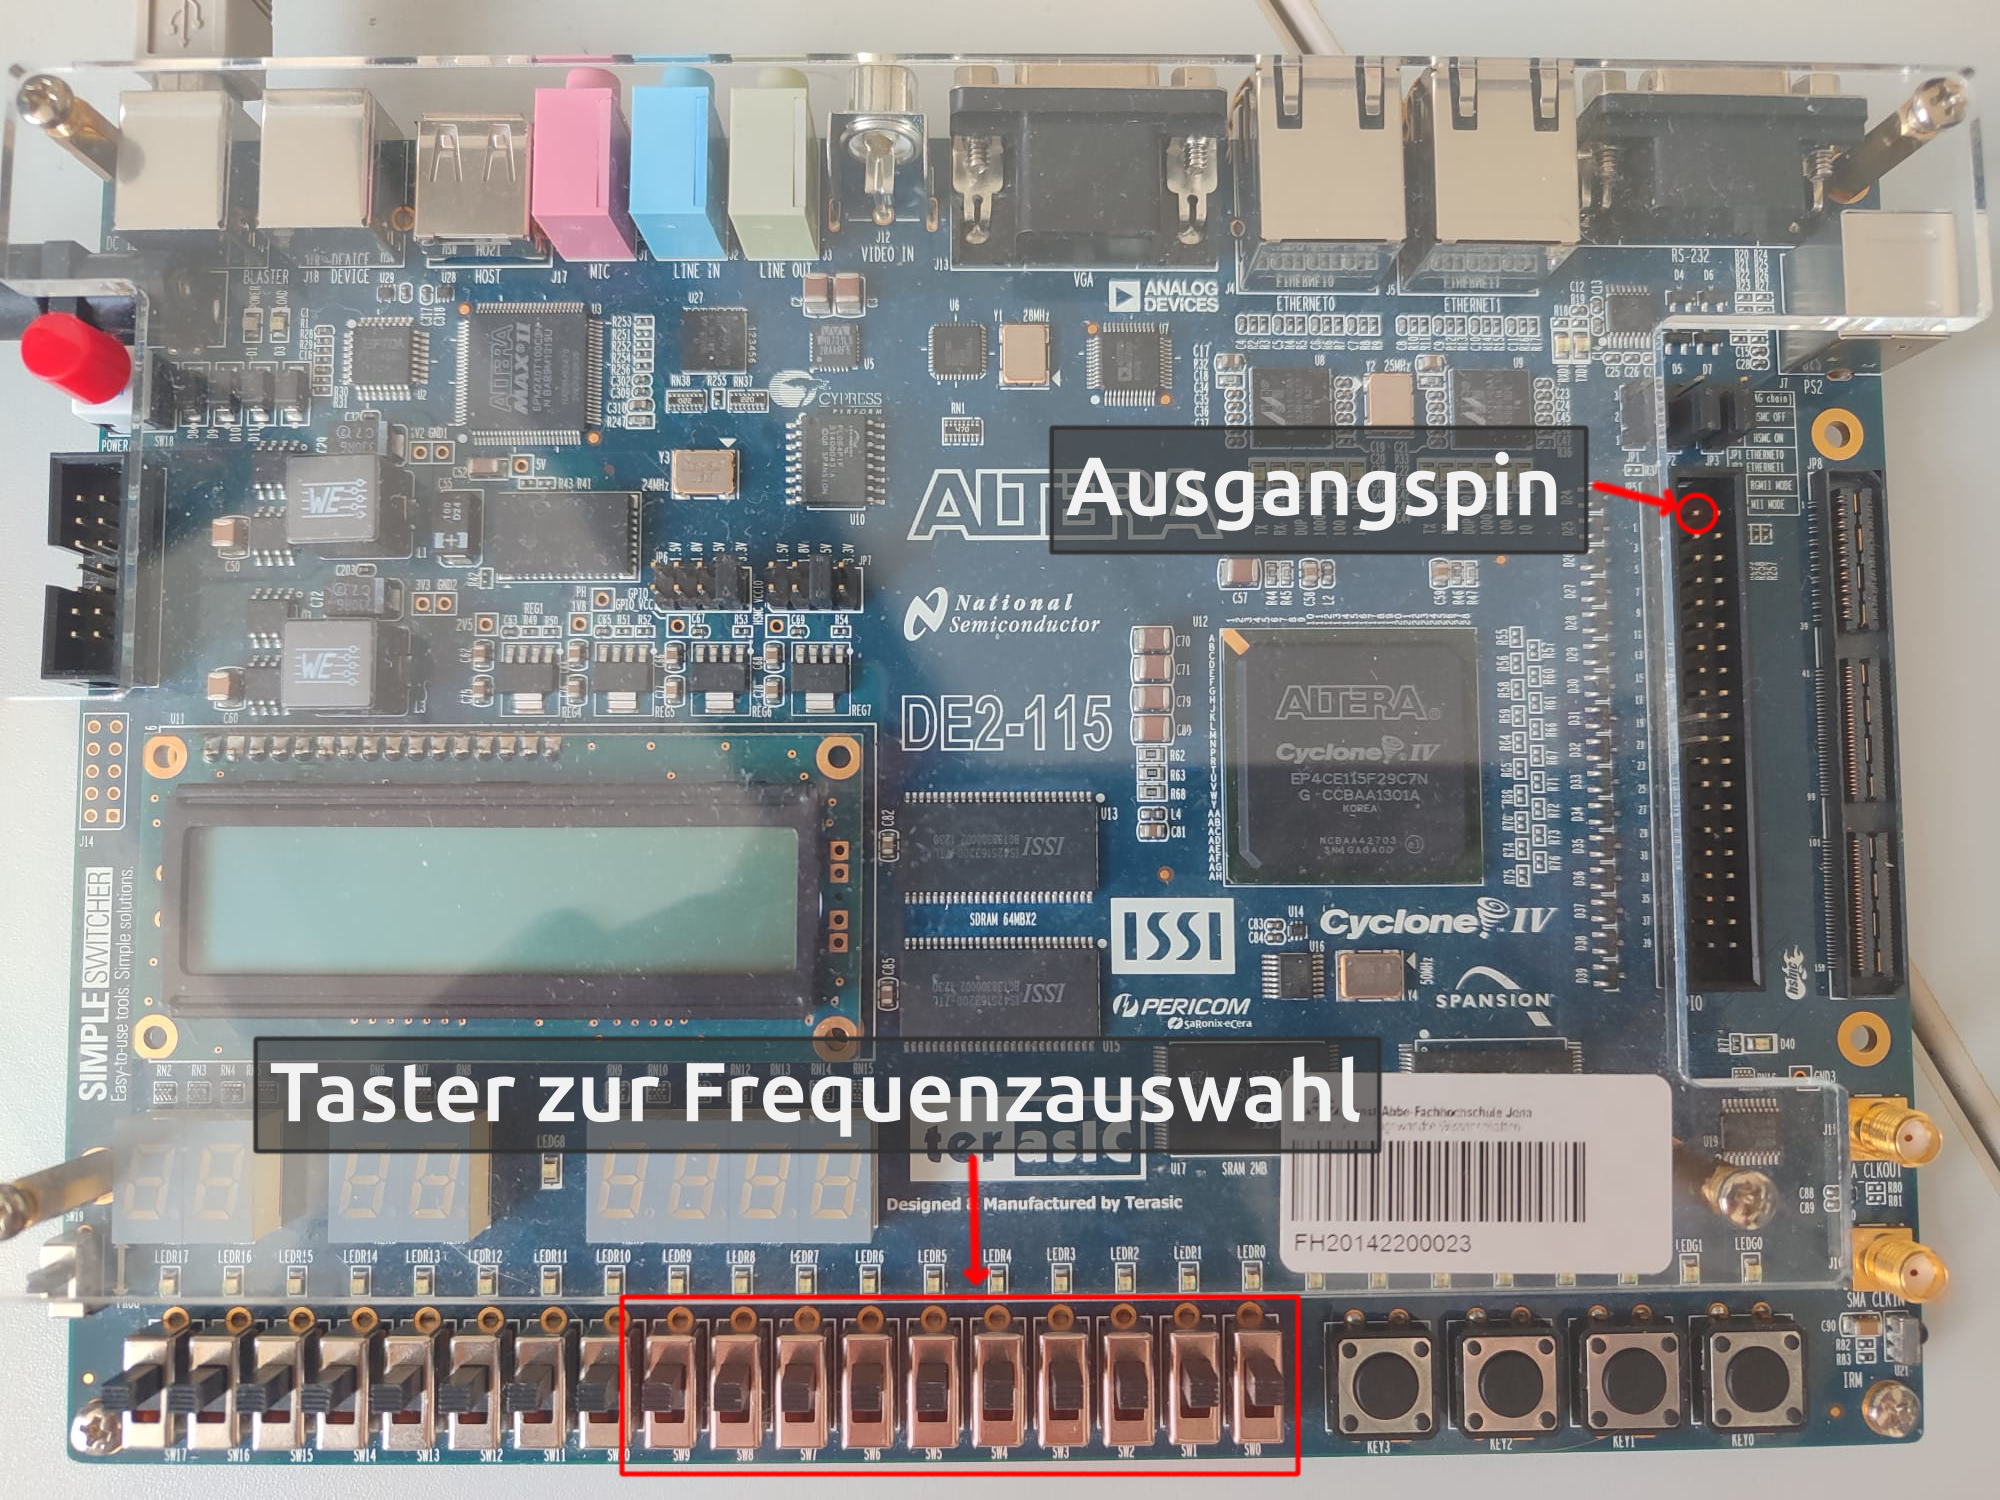
\includegraphics[width=.6\linewidth]{img/io.png}
    \caption{verwendete Ein- und Ausgänge des Boards}
    \label{img_io}
\end{figure}

\subsection{Prinzip der Direct-Digital-Synthesis}
Ein Signalgenerator nach dem Prinzip der Direct-Digital-Synthesis besteht aus mehreren Blöcken.
Der erste Block ist der \textbf{Phasenakkumulator}. Dieser berechnet in jedem Taktschritt den neuen Phasenwert,
indem er den Frequenzauswahlwert auf den aktuellen Zählstand addiert.
Der nächste Teil ist die \textbf{Koeffiziententabelle}. In dieser sind gesampelte Amplitudenwerte der zu 
generierenden Funktion gespeichert.
Der \textbf{PWM-Generator} liest mithilfe des vom Phasenakkumulator generierten
Phasenwerts einen Amplitudenwert aus der Koeffiziententabelle aus und wandelt diesen in ein PWM-Signal um.
Zum Schluss kommt ein \textbf{Tiefpassfilter}, durch den das PWM-Signal in das analoge Signal umgewandelt wird.
Er bildet gemeinsam mit dem PWM-Generator einen einfachen Analog-Digital-Wandler.

\begin{figure}[htbp]
    \centering
    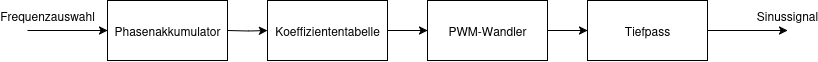
\includegraphics[width=\linewidth]{img/blockschaltbild.png}
    \caption{Blockschaltbild eines DDS-Generators}
    \label{img_blockschaltbild}
\end{figure}

\subsection{Lösungsansatz}


\subsection{Testbench und Use-Cases}
Zur Verifikation der Modelle auf den verschiedenen Ebenen werden zwei Testbenches 
benötigt. Eine für das Modell auf algorithmischer Ebene und eine für die Register-Transfer-Ebene.
Die Testbench auf algorithmischer Ebene erzeugt eine Instanz des Signalgenerators und
wartet eine gewisse Zeit bevor sie sich beendet. Anschließend kann der Verlauf der
Signale ausgewertet werden.
Die Testbench auf Register-Transfer-Ebene beinhaltet zusätzlich noch einen Prozess
zur Generierung des clk-Signals. Auch hier wird eine gewisse Zeit gewartet, bis sich die
Simulation beendet und die Signale ausgewertet werden können.

\noindent Mit den Testbenches werden folgende Use-Cases getestet:
\begin{itemize}
    \item Sinus mit maximal möglicher Frequenz
    \item Sinus mit der mittleren möglichen Frequenz
    \item Sinus mit der minimal möglichen Frequenz
\end{itemize}